\chapter{Additional simulations of the EM algorithm}

\section{Outliers simulations}

Classical methods used for the parameters' estimation, especially the
maximum likelihood estimation (MLE), are sensitive to the presence of
outliers. A naive solution consists in assigning null weights to
observations suspected to be outliers, so that they do not contribute
\footnote{The use of weighted distributions has more general applications.
  It can be used to deal with a component distribution that does not
  fit exactly a Gaussian shape. For instance, to deal with heavy tail
  distributions, more weight can be given to central components and
  less weight to the tails.}. Trimming aberrant observations from the distribution is justified
theoretically by the principle of the \emph{spurious outlier model}
\autocite{gallegos_ritter05}. However, this method is quite stringent,
requiring human expertise or the use of general outlier detection tools
not necessarily adapted to GMM estimation.

Two general approaches for dealing with outliers with a well-defined
theoretical background are the \emph{outliers mixture modelling} and the
\emph{trimming approach}. \emph{Outliers mixture modelling} integrate an
additional component accounting for the outliers in the distribution.
Notably, the \pkg{mclust} \autocite{R-mclust} and \CRANpkg{otrimle} \autocite{R-otrimle}
packages use an improper uniform distribution to model the distribution
of outliers. Unlike \pkg{mclust}, the \pkg{otrimle} package does not
require the user to set in advance the proportion of outliers in the
mixture \autocite{otrimle2016b}. As opposed, in the \emph{trimming approach},
outliers are first removed before the complete estimation of parameters.
Such methods are implemented in \CRANpkg{tclust} \autocite{R-tclust} and
\CRANpkg{oclust} \autocite{R-oclust} packages.

\CRANpkg{tclust} \autocite{R-tclust} uses a robust constrained clustering
method, where the user has to set an upper threshold to the ratio
between the highest and the lowest variability among all components and
a trimming ratio \(\alpha\). It extends the work of
\autocite{garcia-escudero_etal08}, with released constraints on the Gaussian
distribution. First, the maximal degree of affinity, defined in Equation
\eqref{eq:affinity-degree}


\begin{equation}
    D(x_i|\theta)=\max_j \left(p_{j} \varphi_{\zeta_j} (x_i) \right)
\label{eq:affinity-degree}
\end{equation}

is computed for each observation \(x_i\), and corresponds for each point
to the maximum probability to observe it in the distribution, given
parameter \(\theta\). Then, \(\alpha\) observations the least likely to be
observed are trimmed for the estimation of the parameters. When we reach
convergence of the estimated parameter and there is no change in the
outliers identification from one iteration to another, the iterative
algorithm stops. The use of constraints is an additional feature that
avoids building over-dispersed or unbalanced clusters, the highest
constraint of a ratio of 1 yielding clusters with equal sizes. However,
the identification of an observation as aberrant is highly dependant on
the variability constraint and the determination of these two
hyperparameters is complex and highly dependant on the shape of the
distribution. Additionally, a CEM algorithm is used to retrieve the
parameters and the proportion of outliers, for which the MLE, in
contrast to the EM algorithm, is not asymptotically consistent nor
efficient.

Unlike \pkg{tclust}, \CRANpkg{oclust} \autocite{R-oclust} both retrieves the
proportion of outliers and identifies them. To do so, it compares the
complete log-likelihood of the mixture \(\ell(\theta|X)\) with its value
removing one observation \(\ell(\theta | X \setminus X_i)\), for all
observations. Observations are iteratively removed, based on the
assumption that the Kullback-Leibler divergence between the original
log-likelihood and the trimmed log-likelihood
\(\text{KL}\left(\ell(\theta|X)|| \ell(\theta | X \setminus X_i)\right)\)
follows a Beta distribution. At each step, the observation that
maximises the Kullback-Leibler divergence at a statistically significant
threshold is removed. The algorithm stops trimming outliers, when this
measure is not anymore statistically significant. However, the
assumption of a Beta distribution only holds asymptotically and with
non-overlapping clusters.

To integrate the impact of outliers in the estimation, we simulated a
two-components GMM with well-separated and balanced clusters. The
outliers distribution, corresponding to the additional noise component,
was retrieved by randomly selecting \emph{prop.outliers} points out of the
total number of observations and drew their values from an uniform
distribution bounded by an interval five times as big as the 0.05 and
0.95 quantiles of \(f_\theta(X)\). All estimates were obtained comparing
the five reviewed initialisation methods, except with \pkg{otrimle}
which has its own hierarchical clustering initialisation method.

\begin{figure}[p]
\centering
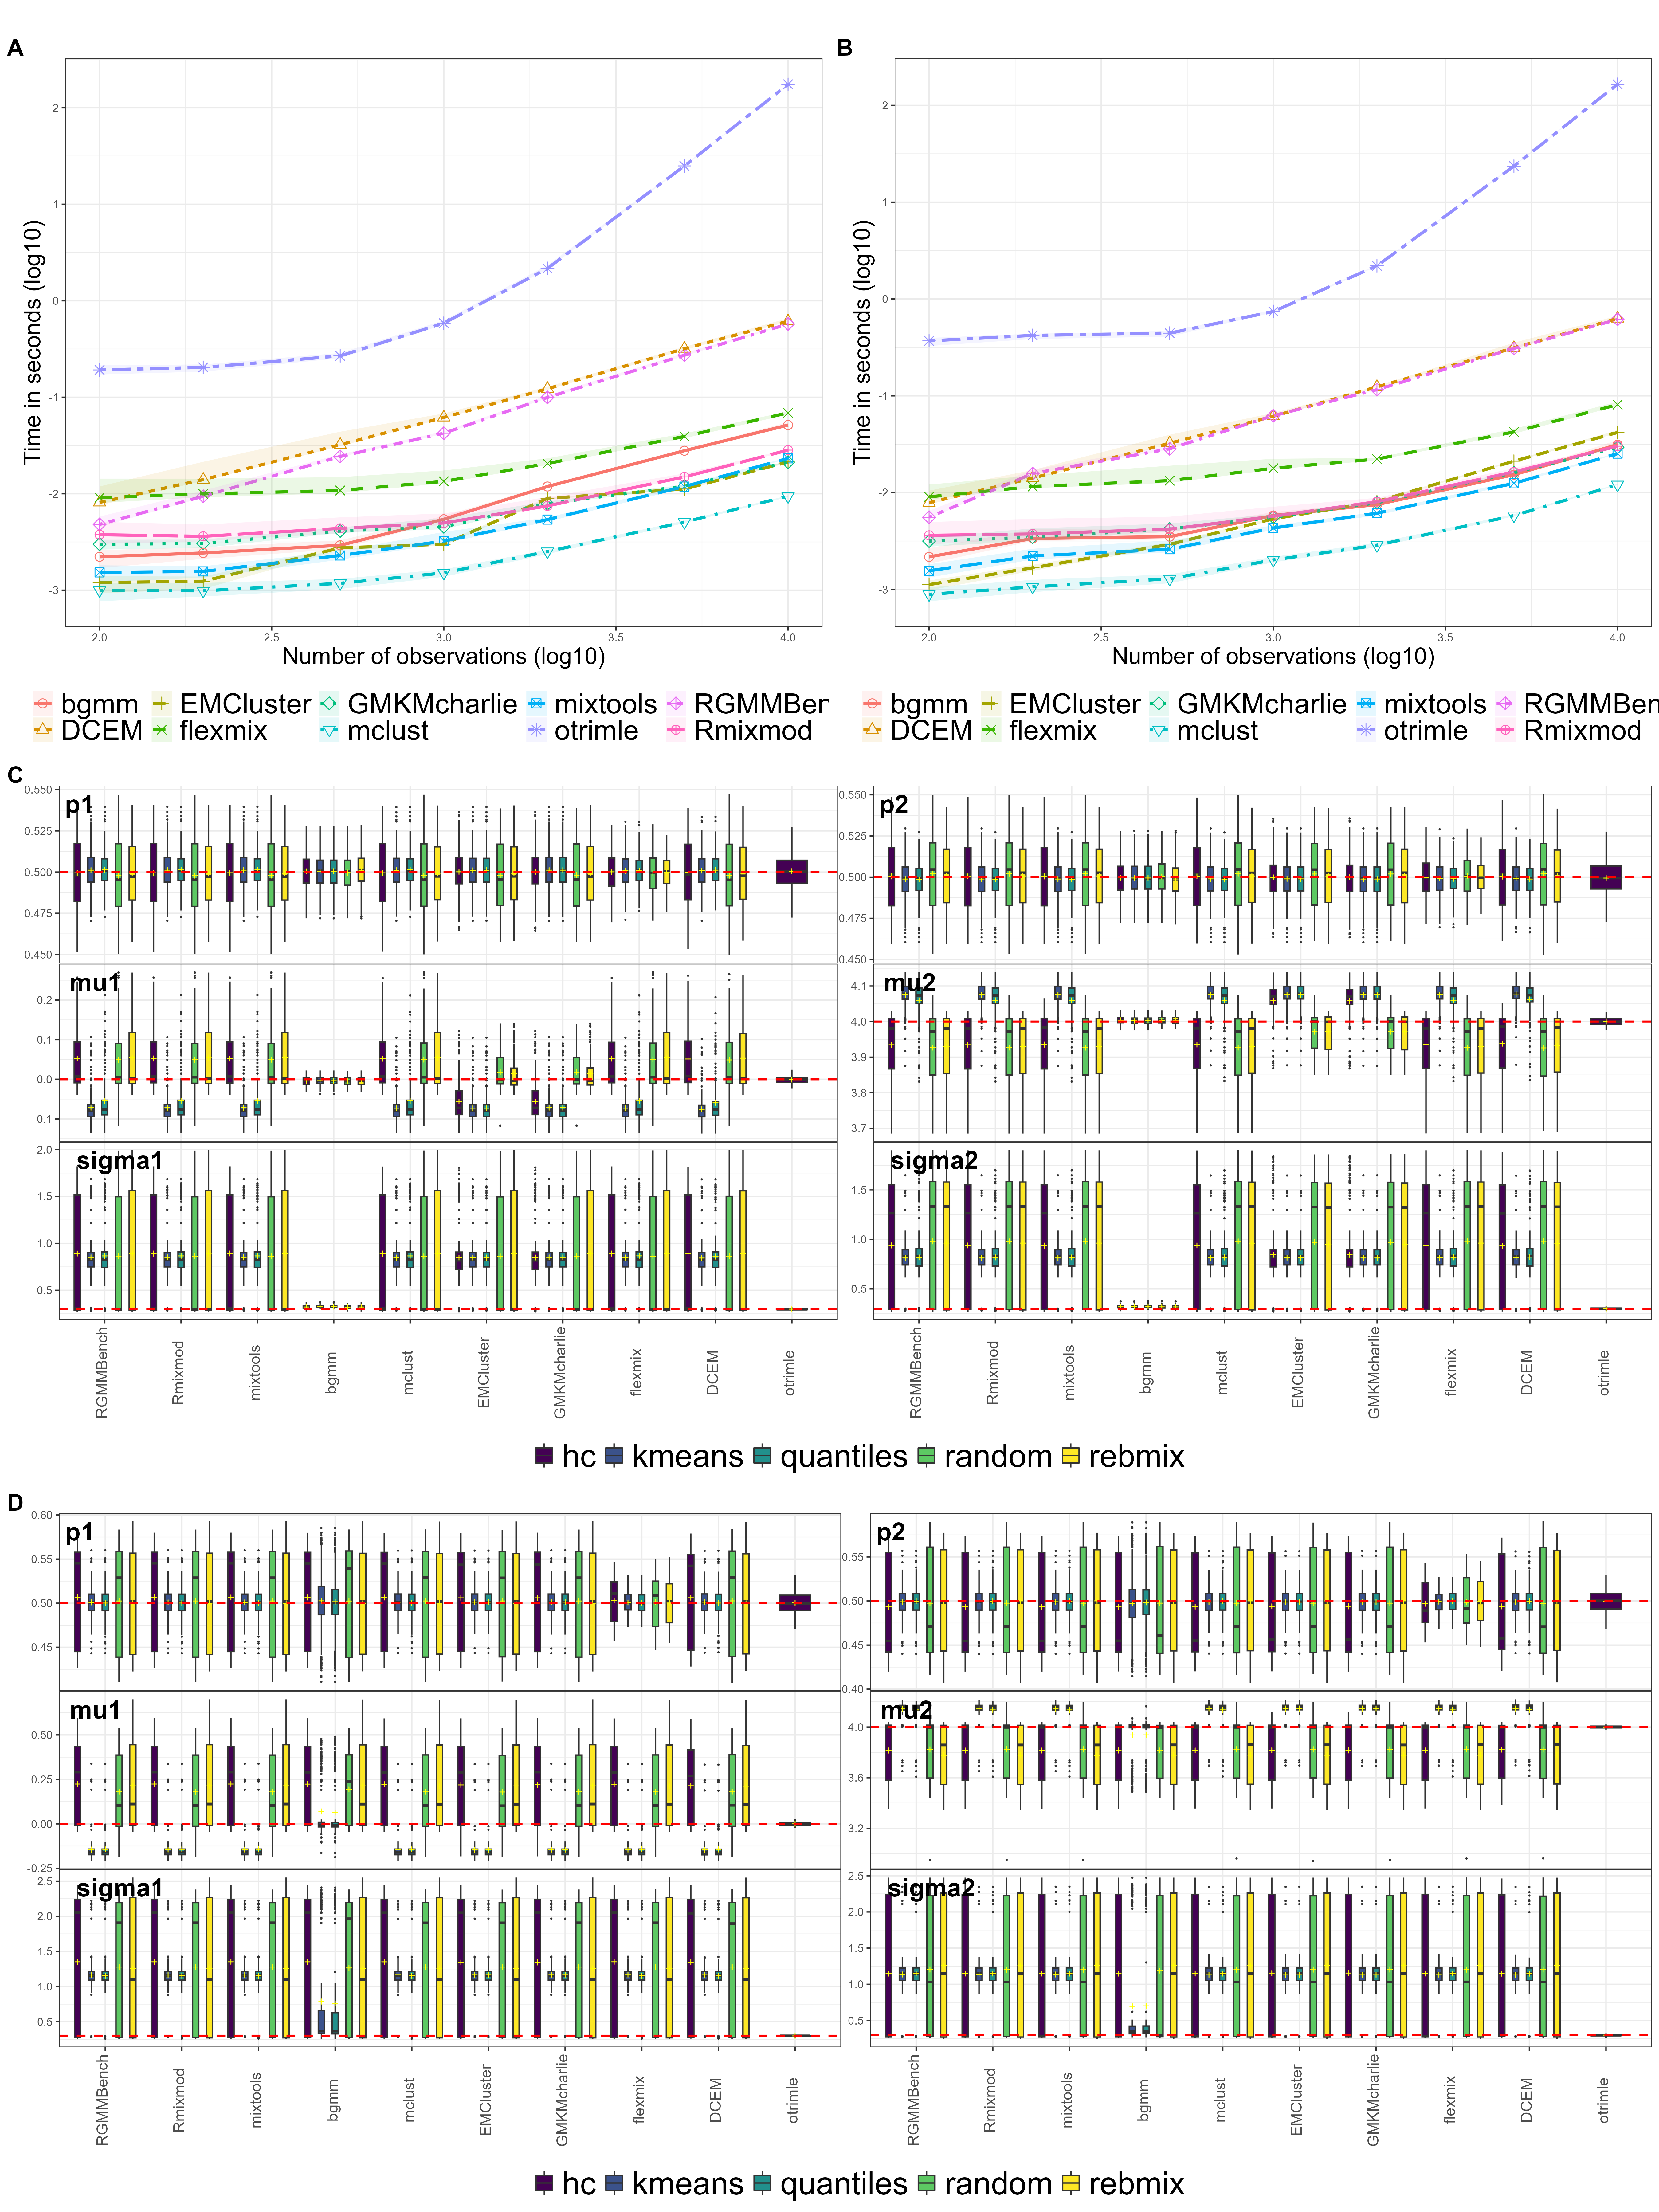
\includegraphics[width=0.9\linewidth,]{figures/outliers} 
\caption{A) Execution times for the nine reviewed packages using hierarchical clustering initialisation, with on the left $2\%$ of outliers in proportion and on the right, $4\%$ of outliers.  B) and C) Boxplots of the estimated parameters with $N=200$ repetitions, $n=2000$ observations and respectively $2\%$ and $4\%$ of outliers. The red dashed horizontal line corresponds to the true value of the parameters.}
\label{fig:outliers}
\end{figure}

The slowest package is \pkg{otrimle}, most of the time being taken by
the initialisation step where proportion and identification of the
outliers is performed. Running times of the other packages are generally
not impacted by the presence of outliers.

Most of the reviewed packages, except the \pkg{bgmm} package, are not
impacted by the choice of initialisation method. Additionally, the
proportions are rather correctly estimated (related to the choice of an
uniform distribution to model outliers), but the reviewed packages tend
to overestimate the true variability of each component, with the worst
results obtained with \pkg{rebmix} initialisation. \pkg{bgmm} sets apart
from the others by its reduced bias on the means and standard deviations
estimated, a feature left undocumented. However, increasing the number
of outliers (Figure \Cref{fig:outliers}, panel C) lead also to biased
estimations for \pkg{bgmm}, while \pkg{otrimle}, a dedicated package, is
still able to correctly estimate the individual parameters of the
components' distributions with a high proportion of outliers. Yet,
analysing the code used to implement the \pkg{bgmm} reveals that there
is no dedicated feature to remove outliers but rather a specific method
used to deal with numerical underflow that artificially increases the
probability of observing outlying distributions.


\section{High-dimensional simulations}
\label{sec:high-dimensional-simulations}


\subsection{Parameters estimation in a high-dimensional context}
\label{subsec:high-dimensional}

However, while parsimonious representations can largely reduce the computational burden, none of them in the general family is able to handle degenerate cases where the number of features, \(D\), exceeds the number of observations \(n\). Likewise situations, when the number of features is consequent, are referred to as high-dimensional, raising the well-known issue of the ``curse of the dimensionality''. Two distinct approaches have been developed in the literature to handle these degenerate cases:

\begin{itemize}
\item
  The most naive approach aims to eliminate the least informative variables by applying a strong Lasso-type penalty on the parameters to be estimated. We only came across such an approach twice among the reviewed R packages, in the specific context of regressions of mixtures (see\pkg{RobMixReg} and \pkg{fmerPack} packages).
\item
  The second category includes a larger diversity of methods, all inspired from the \emph{factor analysis} approach whose paradigm is to consider that all the \(D\) features used to describe the observations can be spanned in a smaller subspace without lose of information. Precisely, the factor analysis theory describes the variability among observed and correlated variables by a substantial lower number of unobserved variables called \emph{factors} or \emph{latent variables}.
  In practice, for a given component \(j\), the diagonal matrix storing the eigenvalues is decomposed into two-blocks. The first upper-right diagonal block, assumed generally of dimension \(d_j \ll D\), stores the largest \(d_j\) eigenvalues and model the variance of the actual data of component \(j\) while the lower-left diagonal block, of dimension \(D-d_j\), stores an unique parameter that can be interpreted as the variance of the residual error terms, constrained to be strictly inferior to the lowest variability of the informative variables. The dimension \(d_j\) can be considered as the intrinsic dimension of the latent subspace of cluster \(j\) spanned by the first \(d_j\) eigenvectors of \(\boldsymbol{Q}_j\). Practically, it is equivalent to consider only the \(d_j^\text{th}\) largest eigenvalues, while discarding the remaining smaller ones.
\end{itemize}

When the sub dimension \(d_j\) is known, a closed version is generally available for the M-step of the EM algorithm, however \(d_j\) is itself an hyperparameter to estimate. Though, \autocite{bouveyron_etal11} has shown that a classical Cattell's scree-test could be used to asymptotically estimate the intrinsic dimension of each cluster. Compared to the previous approach, this method has a strong theoretical background and strong impact on the running times performance.

Taking a concrete use case from the help documentation of the package \pkg{HDclassif}, it enabled to cluster a dataset of 10 classes with 130 observations overall and described in a 1024-dimensional space (consider the famous machine-learning digit recognition problem). Variants of these approaches have been developed in the following packages: \pkg{HDclassif}, \pkg{fabMix}, \pkg{EMMIXmfa} and \pkg{pgmm}. We refer the interested reader to the educational vignette of \pkg{HDclassif} \href{https://rdrr.io/pkg/HDclassif/man/HDclassif-package.html}{HDclassif} and papers \autocite{mcnicholas_murphy08}--\autocite{mcnicholas_murphy10}.

Historically, the first mention of a probabilistic framework with an application to dimension reduction in the context of finite mixture models goes back to \autocite{tipping_bishop99}, based on principal component analysis. \autocite{mclachlan_etal03} and \autocite{mclachlan_peel00a} extend this original model by postulating that the distribution of the data within any latent class could be described using the tools of the factor analysis field\footnote{Although principal component analysis and factor analysis are closely related, we can differentiate both approaches by their differing objective: while PCA seeks to capture the overall variability of the dataset, factor analysis focuses on describing the intra-variability between covariates. In practice, the differences between the two approaches are minor, we can notably show that the output of PCA is one of the solutions suggested by standard factor analysis.} Finally, building on the parsimonious parametrisations already theorised for GMMs (see previous section) , \autocite{mcnicholas_murphy08}, \autocite{mcnicholas_etal10} and \autocite{bouveyron_etal07} proposed a variety of constraints, but this time directly defined on the projected subspace. Since all methods based on factor analysis provide a transition matrix, using the two or three most informative eigen values and their associated eigen vectors in order to project the dataset on a smaller subspace provides a simple visualisation tool for representing high dimensional datasets.
However, this method may is not suitable for unravelling the clustering structure. Instead, \emph{the GMMDR method}, first proposed by \autocite{scrucca10} and implemented in the \texttt{MclustDR} function, from \pkg{mclust} package, aims at recovering the subspace that best captures the underlying latent clustering structure (we notably expect invariance of the global overlap in the sampling space and the corresponding projected subspace). More precisely, the main objective of the GMMDR technique is to infer the global \emph{change-of-basis matrix} \(\boldsymbol{Q}\) that minimises the differences in the a posteriori probabilities of assigning each observation \(i\) to a given cluster \(s_i\), knowing the value of the vector of observed covariates \(\boldsymbol{x}_i\). Namely, we are looking for the orientation matrix \(\boldsymbol{Q}\) that maximally ensures the following objective (Eq. \eqref{eq:GMMDR}):

\begin{equation}
 \hat{\boldsymbol{Q}} = \arg \max_{\boldsymbol{Q}} \,  \left(\mathbb{P}_{\theta} (S_i=j | \boldsymbol{X} =\boldsymbol{x}_i) = \mathbb{P}_{\theta} (S_i=j | \boldsymbol{X} \boldsymbol{Q}) \right)
\text{ such that } S \perp \boldsymbol{X} | \boldsymbol{X} \boldsymbol{Q}
    \label{eq:GMMDR}
\end{equation}

This procedure itself derives from the \emph{sliced inverse regression} algorithm \autocite{li91}, but instead of conditioning on the known response variable, GMMDR conditions on the estimated MAP cluster assignments. Since the solution returned by the following optimization problem is not unique, we generally constrain the projection matrix to be orthonormal (any of the vectors forming the basis are pairwise orthogonal, and individually of norm 1).

About the practical implementation, the intrinsic dimension \(d_j\) for each cluster \(j\) is itself a hyperparameter inferred independently from the GMM estimation itself. While a variety of methods from the field of factor analysis, enumerated in \href{https://en.wikipedia.org/wiki/Factor_analysis\#Criteria_for_determining_the_number_of_factors}{Factor criteria selection}, have been developed to estimate the intrinsic dimension, to our knowledge, only two of them have been implemented in CRAN packages: the \emph{Cattell's scree-test} \autocite{cattell66} or the dimension selection graph using one of the \emph{penalty metric} discussed in paper \autocite{berge_etal12}. However, while \pkg{HDclassif} natively implements a performance criterion method for determining the dimension of the spanning spak;kgk;gkgkkgggce, performed under the hood by function \texttt{mixsmsn::hdcc}, none of the other packages evaluated implemented a dimension selection feature. Instead, we infer it for each of the packages dedicated to high-dimensionality with HDclassif, using using the so-called model ``AkjBkQkD'', for which the intrinsic dimension is common to all components but the characteristics unique for each component Finally, we use among all supplied parametrisations, the least constrained one. Namely, we used the model \texttt{AkjBkQkDk} with HDclassif, in which not only the individual features of the covariance matrix but also the spanning dimension are unique for each cluster, and function \texttt{mcfa} of the \pkg{ EMMIXmfa} package, in which the \emph{transition matrix} is common to all components.


\subsection{Figures and Tables in the HD simulation}
\label{figures-hd-simulation}

Table below (\Cref{tab:parameter-configuration-HD}) lists the complete set of parameters used to simulate Gaussian distributions in the high dimensional benchmark:

\begin{table}[!h]

\caption{\label{tab:parameter-configuration-HD}The 16 parameter configurations tested to generate the samples in a high dimensional context. The first digit of each ID index refers
      to an unique parameter configuration (identified by its level of overlap, entropy and topological structure, either circular or ellipsoidal,
      of the covariance matrix, while the lowercase letter depicts the number of observations, a) with $n=200$ and b) with $n=2000$.}
\centering
\resizebox{\linewidth}{!}{
\begin{tabular}[t]{ccccc}
\toprule
\textbf{ID} & \textbf{OVL} & \textbf{\makecell[r]{Number of \\observations}} & \textbf{Proportions} & \textbf{Spherical}\\
\midrule
HD1a & 1e-04 & 200 & 0.5 / 0.5 & 
\includegraphics[scale=0.05]{figures/green_tick.png}\\
\midrule
HD1b & 1e-04 & 2000 & 0.5 / 0.5 & 
\includegraphics[scale=0.05]{figures/green_tick.png}\\
\midrule
HD2a & 1e-04 & 200 & 0.19 / 0.81 & 
\includegraphics[scale=0.05]{figures/green_tick.png}\\
\midrule
HD2b & 1e-04 & 2000 & 0.19 / 0.81 & 
\includegraphics[scale=0.05]{figures/green_tick.png}\\
\midrule
HD3a & 1e-04 & 200 & 0.5 / 0.5 & 
\includegraphics[scale=0.05]{figures/red_cross.png}\\
\midrule
\addlinespace
HD3b & 1e-04 & 2000 & 0.5 / 0.5 & 
\includegraphics[scale=0.05]{figures/red_cross.png}\\
\midrule
HD4a & 1e-04 & 200 & 0.21 / 0.79 & 
\includegraphics[scale=0.05]{figures/red_cross.png}\\
\midrule
HD4b & 1e-04 & 2000 & 0.21 / 0.79 & 
\includegraphics[scale=0.05]{figures/red_cross.png}\\
\midrule
HD5a & 2e-01 & 200 & 0.5 / 0.5 & 
\includegraphics[scale=0.05]{figures/green_tick.png}\\
\midrule
HD5b & 2e-01 & 2000 & 0.5 / 0.5 & 
\includegraphics[scale=0.05]{figures/green_tick.png}\\
\midrule
\addlinespace
HD6a & 2e-01 & 200 & 0.15 / 0.85 & 
\includegraphics[scale=0.05]{figures/green_tick.png}\\
\midrule
HD6b & 2e-01 & 2000 & 0.15 / 0.85 & 
\includegraphics[scale=0.05]{figures/green_tick.png}\\
\midrule
HD7a & 2e-01 & 200 & 0.5 / 0.5 & 
\includegraphics[scale=0.05]{figures/red_cross.png}\\
\midrule
HD7b & 2e-01 & 2000 & 0.5 / 0.5 & 
\includegraphics[scale=0.05]{figures/red_cross.png}\\
\midrule
HD8a & 2e-01 & 200 & 0.69 / 0.31 & 
\includegraphics[scale=0.05]{figures/red_cross.png}\\
\midrule
\addlinespace
HD8b & 2e-01 & 2000 & 0.69 / 0.31 & 
\includegraphics[scale=0.05]{figures/red_cross.png}\\
\midrule
\bottomrule
\end{tabular}}
\end{table}

\newpage

\begin{table}[!htbp]

\caption{\label{tab:HD-separated-unbalanced-ellipsoidal-pdf}MSE and Bias associated to scenario HD4a, in Table
      \Cref{tab:parameter-configuration-HD} (unbalanced, separated and ellipsoidal components).}
\centering
\resizebox{\linewidth}{!}{
\begin{tabu} to \linewidth {>{}l>{}l>{}r>{}r>{}r>{}r>{}r>{}r>{}r}
\toprule
\multicolumn{1}{c}{\textbf{Package}} & \multicolumn{1}{c}{\textbf{\makecell[c]{Initialisation\\Method}}} & \multicolumn{1}{c}{\textbf{\makecell[r]{Global \\ MSE $p$}}} & \multicolumn{1}{c}{\textbf{\makecell[l]{Global\\MSE $\mu$}}} & \multicolumn{1}{c}{\textbf{\makecell[c]{Global\\MSE $\sigma$}}} & \multicolumn{1}{c}{\textbf{\makecell[r]{Global \\ Bias $p$}}} & \multicolumn{1}{c}{\textbf{\makecell[l]{Global\\Bias $\mu$}}} & \multicolumn{1}{c}{\textbf{\makecell[c]{Global\\Bias $\sigma$}}} & \multicolumn{1}{c}{\textbf{$\%$ Success}}\\
\midrule
 & hc & \textcolor{green}{0.0333} & \textcolor{green}{0.0212} & \textcolor{green}{0.0106} & \textcolor{black}{0.0020} & \textcolor{green}{0.056} & \textcolor{black}{0.097} & \textcolor{green}{100}\\

 & kmeans & \textcolor{green}{0.0333} & \textcolor{green}{0.0212} & \textcolor{green}{0.0106} & \textcolor{black}{0.0020} & \textcolor{green}{0.056} & \textcolor{black}{0.097} & \textcolor{green}{100}\\

\multirow{-3}{*}{\raggedright\arraybackslash \textbf{mixtools / Rmixmod / RGMMBench}} & rebmix & \textcolor{black}{0.3244} & \textcolor{black}{0.1980} & \textcolor{black}{0.0845} & \textcolor{black}{0.0720} & \textcolor{black}{0.395} & \textcolor{black}{0.535} & \textcolor{black}{98}\\
\cmidrule{1-9}
 & hc & \textcolor{green}{0.0333} & \textcolor{green}{0.0212} & \textcolor{green}{0.0106} & \textcolor{black}{0.0020} & \textcolor{green}{0.056} & \textcolor{black}{0.097} & \textcolor{green}{100}\\

 & kmeans & \textcolor{green}{0.0333} & \textcolor{green}{0.0212} & \textcolor{green}{0.0106} & \textcolor{black}{0.0020} & \textcolor{green}{0.056} & \textcolor{black}{0.097} & \textcolor{green}{100}\\

\multirow{-3}{*}{\raggedright\arraybackslash \textbf{mclust / flexmix / GMKMcharlie}} & rebmix & \textcolor{black}{0.2553} & \textcolor{black}{0.1444} & \textcolor{black}{0.0924} & \textcolor{black}{0.0470} & \textcolor{black}{0.364} & \textcolor{black}{0.596} & \textcolor{black}{85}\\
\cmidrule{1-9}
 & hc & \textcolor{black}{0.0337} & \textcolor{black}{0.0214} & \textcolor{black}{0.0107} & \textcolor{black}{0.0070} & \textcolor{black}{0.064} & \textcolor{green}{0.096} & \textcolor{green}{100}\\

 & kmeans & \textcolor{black}{0.0338} & \textcolor{black}{0.0216} & \textcolor{green}{0.0106} & \textcolor{black}{0.0074} & \textcolor{black}{0.064} & \textcolor{green}{0.096} & \textcolor{green}{100}\\

\multirow{-3}{*}{\raggedright\arraybackslash \textbf{bgmm}} & rebmix & \textcolor{black}{0.4818} & \textcolor{black}{0.1152} & \textcolor{black}{0.3442} & \textcolor{black}{0.0320} & \textcolor{black}{0.223} & \textcolor{black}{2.329} & \textcolor{black}{94}\\
\cmidrule{1-9}
 & hc & \textcolor{green}{0.0333} & \textcolor{green}{0.0212} & \textcolor{black}{0.0107} & \textcolor{black}{0.0023} & \textcolor{green}{0.056} & \textcolor{green}{0.096} & \textcolor{green}{100}\\

 & kmeans & \textcolor{black}{0.0334} & \textcolor{black}{0.0213} & \textcolor{green}{0.0106} & \textcolor{green}{0.0018} & \textcolor{green}{0.056} & \textcolor{green}{0.096} & \textcolor{green}{100}\\

\multirow{-3}{*}{\raggedright\arraybackslash \textbf{EMCluster}} & rebmix & \textcolor{black}{1.5983} & \textcolor{black}{1.0992} & \textcolor{red}{0.3794} & \textcolor{black}{0.3100} & \textcolor{black}{2.018} & \textcolor{black}{2.575} & \textcolor{black}{84}\\
\midrule
\cmidrule{1-9}
 & hc & \textcolor{red}{8.4062} & \textcolor{red}{8.3936} & \textcolor{black}{0.0111} & \textcolor{black}{0.0020} & \textcolor{red}{10.426} & \textcolor{black}{0.149} & \textcolor{green}{100}\\

 & kmeans & \textcolor{black}{7.9407} & \textcolor{black}{7.9282} & \textcolor{black}{0.0111} & \textcolor{black}{0.0019} & \textcolor{black}{10.081} & \textcolor{black}{0.149} & \textcolor{green}{100}\\

\multirow{-3}{*}{\raggedright\arraybackslash \textbf{HDclassif}} & rebmix & \textcolor{black}{7.9803} & \textcolor{black}{7.9514} & \textcolor{black}{0.0273} & \textcolor{black}{0.0044} & \textcolor{black}{10.128} & \textcolor{black}{0.262} & \textcolor{black}{84}\\
\cmidrule{1-9}
 & hc & \textcolor{black}{4.0605} & \textcolor{black}{3.3317} & \textcolor{black}{0.3357} & \textcolor{red}{0.6500} & \textcolor{black}{5.757} & \textcolor{black}{2.772} & \textcolor{black}{95}\\

 & kmeans & \textcolor{black}{3.8790} & \textcolor{black}{3.2175} & \textcolor{black}{0.3372} & \textcolor{black}{0.5400} & \textcolor{black}{5.781} & \textcolor{red}{2.777} & \textcolor{black}{96}\\

\multirow{-3}{*}{\raggedright\arraybackslash \textbf{EMMIXmfa}} & rebmix & \textcolor{black}{4.0127} & \textcolor{black}{3.2715} & \textcolor{black}{0.3337} & \textcolor{black}{0.5700} & \textcolor{black}{5.680} & \textcolor{black}{2.757} & \textcolor{red}{80}\\
\bottomrule
\end{tabu}}
\end{table}

\newpage

\begin{figure}[htbp]

{\centering \includegraphics[width=0.6\linewidth,]{figures/HD-separated-unbalanced-ellipsoidal} 

}

\caption{Results of scenario HD4a) in Table \Cref{tab:parameter-configuration-HD} (unbalanced, overlapping and negative correlated components), organised as such:
The panel A displays the bivariate factorial projection of a random sample drawn from the 10-dimensional multivariate Gaussian distribution parametrised by Table \Cref{tab:parameter-configuration-HD}. Each component is associated to a specific color, a centroid whose coordinates are given by the mean components' elements in the bivariate projected space and a $95\%$ confidence ellipse. Arrows represent the correlation circle of the dimensional variables.
 Both panels were displayed respectively using functions \texttt{factoextra::fviz\_eig} and \texttt{factoextra::fviz\_pca\_biplot} while the underlying computations proceed from the principal component analysis performed by \texttt{ade4::dudi.pca} preceded by standard scaling of the sampling dataset.
The panel B pictures the \emph{parallel distribution plots} from a random sampling of $n=100$ observations, generated using \texttt{GGally::ggparcoord}, and representing the coordinates of each simulated data point in 10 dimensions.
The running times are displayed in Panel C with the \emph{k}-means initialisation. The number of observations (x-axis) and the running time (y-axis) is in $\log(10)$ scale.
The distributions of the Hellinger distances are computed for each component in Panel D, each initialisation method and each package with respect to the true Gaussian distribution expected for each component.
In panel E we represent the boxplots associated with the distribution of some of the estimates. Since it was impractical to represent all of the $k + kD + k\frac{D \times (D+1)}{2}$ with $k=2$ and $D=10$ parameters, we only represent the first component's mean, two first components' variances and their covariance term.}\label{fig:HD-separated-unbalanced-ellipsoidal-plot}
\end{figure}

\newpage

\begin{table}[!htbp]

\caption{\label{tab:HD-overlapping-balanced-ellipsoidal-pdf}MSE and Bias associated to scenario HD7a, in Table
      \Cref{tab:parameter-configuration-HD} (balanced, overlapping and ellipsoidal components).}
\centering
\resizebox{\linewidth}{!}{
\begin{tabu} to \linewidth {>{}l>{}l>{}r>{}r>{}r>{}r>{}r>{}r>{}r}
\toprule
\multicolumn{1}{c}{\textbf{Package}} & \multicolumn{1}{c}{\textbf{\makecell[c]{Initialisation\\Method}}} & \multicolumn{1}{c}{\textbf{\makecell[r]{Global \\ MSE $p$}}} & \multicolumn{1}{c}{\textbf{\makecell[l]{Global\\MSE $\mu$}}} & \multicolumn{1}{c}{\textbf{\makecell[c]{Global\\MSE $\sigma$}}} & \multicolumn{1}{c}{\textbf{\makecell[r]{Global \\ Bias $p$}}} & \multicolumn{1}{c}{\textbf{\makecell[l]{Global\\Bias $\mu$}}} & \multicolumn{1}{c}{\textbf{\makecell[c]{Global\\Bias $\sigma$}}} & \multicolumn{1}{c}{\textbf{$\%$ Success}}\\
\midrule
 & hc & \textcolor{black}{5.8544} & \textcolor{black}{2.2153} & \textcolor{black}{3.5586} & \textcolor{black}{0.0450} & \textcolor{black}{2.084} & \textcolor{black}{6.704} & \textcolor{green}{100}\\

 & kmeans & \textcolor{black}{5.4773} & \textcolor{black}{1.9490} & \textcolor{black}{3.4819} & \textcolor{green}{0.0086} & \textcolor{black}{2.323} & \textcolor{black}{6.861} & \textcolor{green}{100}\\

\multirow{-3}{*}{\raggedright\arraybackslash \textbf{mixtools / Rmixmod / RGMMBench}} & rebmix & \textcolor{black}{6.9243} & \textcolor{black}{2.5185} & \textcolor{black}{4.2898} & \textcolor{black}{0.0620} & \textcolor{black}{2.670} & \textcolor{black}{7.626} & \textcolor{black}{97}\\
\cmidrule{1-9}
 & hc & \textcolor{black}{6.0584} & \textcolor{black}{2.4737} & \textcolor{black}{3.5198} & \textcolor{black}{0.0180} & \textcolor{black}{2.565} & \textcolor{black}{7.624} & \textcolor{green}{100}\\

 & kmeans & \textcolor{black}{5.6388} & \textcolor{black}{2.1597} & \textcolor{black}{3.4549} & \textcolor{black}{0.0140} & \textcolor{black}{2.744} & \textcolor{black}{8.266} & \textcolor{green}{100}\\

\multirow{-3}{*}{\raggedright\arraybackslash \textbf{mclust / flexmix / GMKMcharlie}} & rebmix & \textcolor{black}{6.5397} & \textcolor{black}{2.4738} & \textcolor{black}{3.9661} & \textcolor{black}{0.0700} & \textcolor{black}{2.774} & \textcolor{black}{7.764} & \textcolor{black}{93}\\
\cmidrule{1-9}
 & hc & \textcolor{black}{9.5015} & \textcolor{black}{5.1348} & \textcolor{black}{4.1086} & \textcolor{black}{0.1000} & \textcolor{black}{3.720} & \textcolor{black}{10.310} & \textcolor{green}{100}\\

 & kmeans & \textcolor{black}{8.7930} & \textcolor{black}{4.7119} & \textcolor{black}{3.8693} & \textcolor{black}{0.1500} & \textcolor{black}{3.932} & \textcolor{black}{10.108} & \textcolor{green}{100}\\

\multirow{-3}{*}{\raggedright\arraybackslash \textbf{bgmm}} & rebmix & \textcolor{black}{10.3630} & \textcolor{black}{5.6474} & \textcolor{black}{4.4026} & \textcolor{red}{0.2700} & \textcolor{black}{3.798} & \textcolor{black}{10.049} & \textcolor{black}{97}\\
\cmidrule{1-9}
 & hc & \textcolor{black}{6.4022} & \textcolor{black}{2.8255} & \textcolor{black}{3.5124} & \textcolor{black}{0.0120} & \textcolor{black}{3.141} & \textcolor{black}{9.086} & \textcolor{green}{100}\\

 & kmeans & \textcolor{black}{6.4333} & \textcolor{black}{2.8740} & \textcolor{black}{3.5523} & \textcolor{black}{0.0110} & \textcolor{black}{4.210} & \textcolor{red}{11.007} & \textcolor{green}{100}\\

\multirow{-3}{*}{\raggedright\arraybackslash \textbf{EMCluster}} & rebmix & \textcolor{black}{6.5527} & \textcolor{black}{2.9643} & \textcolor{black}{3.4862} & \textcolor{black}{0.0580} & \textcolor{black}{3.051} & \textcolor{black}{9.253} & \textcolor{black}{93}\\
\midrule
\cmidrule{1-9}
 & hc & \textcolor{black}{15.9010} & \textcolor{red}{11.5382} & \textcolor{black}{4.2950} & \textcolor{black}{0.1400} & \textcolor{black}{10.846} & \textcolor{black}{10.100} & \textcolor{green}{100}\\

 & kmeans & \textcolor{black}{15.3377} & \textcolor{black}{10.9441} & \textcolor{black}{4.3716} & \textcolor{black}{0.0087} & \textcolor{red}{10.990} & \textcolor{black}{10.771} & \textcolor{green}{100}\\

\multirow{-3}{*}{\raggedright\arraybackslash \textbf{HDclassif}} & rebmix & \textcolor{red}{16.1231} & \textcolor{black}{11.1103} & \textcolor{red}{4.9113} & \textcolor{black}{0.1600} & \textcolor{black}{10.761} & \textcolor{black}{10.513} & \textcolor{black}{93}\\
\cmidrule{1-9}
 & hc & \textcolor{black}{4.8606} & \textcolor{black}{1.6546} & \textcolor{black}{3.1856} & \textcolor{black}{0.0160} & \textcolor{black}{2.030} & \textcolor{black}{7.395} & \textcolor{red}{15}\\

 & kmeans & \textcolor{green}{4.4039} & \textcolor{green}{1.4129} & \textcolor{green}{2.9701} & \textcolor{black}{0.0260} & \textcolor{green}{1.734} & \textcolor{green}{6.236} & \textcolor{black}{21}\\

\multirow{-3}{*}{\raggedright\arraybackslash \textbf{EMMIXmfa}} & rebmix & \textcolor{black}{5.0984} & \textcolor{black}{2.0057} & \textcolor{black}{3.0689} & \textcolor{black}{0.0470} & \textcolor{black}{2.314} & \textcolor{black}{7.613} & \textcolor{black}{16}\\
\bottomrule
\end{tabu}}
\end{table}

\newpage

\begin{figure}[htbp]

{\centering \includegraphics[width=0.8\linewidth,]{figures/HD-overlapping-balanced-ellipsoidal} 

}

\caption{Results of scenario HD7a) in Table \Cref{tab:parameter-configuration-HD} (balanced and overlapping components, with full covariance structure), with the same layout as Figure \Cref{fig:HD-separated-unbalanced-ellipsoidal-plot}.}\label{fig:HD-overlapping-balanced-ellipsoidal-plot}
\end{figure}

\newpage

\begin{table}[!htbp]

\caption{\label{tab:HD-overlapping-spherical-pdf}MSE and Bias associated to scenarios HD5a) and HD6a), in Table
\Cref{tab:parameter-configuration-HD} (overlapping and spherical-distributed components). We delimite each scenario by doubled backslashes with respectively balanced and unbalanced clusters.}
\centering
\resizebox{\linewidth}{!}{
\begin{tabu} to \linewidth {>{}l>{}l>{}l>{}l>{}l>{}l>{}l>{}l>{}l}
\toprule
\multicolumn{1}{c}{\textbf{Package}} & \multicolumn{1}{c}{\textbf{\makecell[c]{Initialisation\\Method}}} & \multicolumn{1}{c}{\textbf{\makecell[r]{Global \\ MSE $p$}}} & \multicolumn{1}{c}{\textbf{\makecell[l]{Global\\MSE $\mu$}}} & \multicolumn{1}{c}{\textbf{\makecell[c]{Global\\MSE $\sigma$}}} & \multicolumn{1}{c}{\textbf{\makecell[r]{Global \\ Bias $p$}}} & \multicolumn{1}{c}{\textbf{\makecell[l]{Global\\Bias $\mu$}}} & \multicolumn{1}{c}{\textbf{\makecell[c]{Global\\Bias $\sigma$}}} & \multicolumn{1}{c}{\textbf{$\%$ Success}}\\
\midrule
 & hc & \textcolor{black}{4.2772 // 19.5172} & \textcolor{black}{0.9198 // 1.9835} & \textcolor{black}{3.3027 // 17.4943} & \textcolor{black}{0.017 // 0.069} & \textcolor{black}{0.995 // 0.6} & \textcolor{black}{3.571 // 4.381} & \textcolor{green}{100 // 100}\\

 & kmeans & \textcolor{black}{3.9776 // 17.2212} & \textcolor{black}{0.8279 // 1.6336} & \textcolor{black}{3.1111 // 15.5684} & \textcolor{black}{0.072 // 0.069} & \textcolor{black}{0.841 // 0.82} & \textcolor{black}{3.023 // 5.034} & \textcolor{green}{100 // 100}\\

\multirow{-3}{*}{\raggedright\arraybackslash \textbf{mixtools / Rmixmod / RGMMBench}} & rebmix & \textcolor{black}{9.3136 // 25.8028} & \textcolor{black}{2.7793 // 4.2893} & \textcolor{black}{6.4009 // 21.3519} & \textcolor{black}{0.15 // 0.22} & \textcolor{black}{3.619 // 2.507} & \textcolor{black}{9.061 // 11.826} & \textcolor{black}{96 // 80}\\
\cmidrule{1-9}
 & hc & \textcolor{black}{2.9743 // 18.1175} & \textcolor{black}{0.5862 // 1.7729} & \textcolor{black}{2.3612 // 16.3168} & \textcolor{green}{0.024 // 0.057} & \textcolor{green}{0.449 // 0.514} & \textcolor{green}{2.127 // 4.412} & \textcolor{green}{100 // 100}\\

 & kmeans & \textcolor{black}{2.5629 // 15.2959} & \textcolor{green}{0.4642 // 1.5608} & \textcolor{black}{2.0855 // 13.7206} & \textcolor{black}{0.085 // 0.086} & \textcolor{black}{0.671 // 1.047} & \textcolor{black}{1.67 // 5.801} & \textcolor{green}{100 // 100}\\

\multirow{-3}{*}{\raggedright\arraybackslash \textbf{mclust / flexmix / GMKMcharlie}} & rebmix & \textcolor{black}{8.2907 // 23.7588} & \textcolor{black}{2.6468 // 4.1629} & \textcolor{black}{5.5421 // 19.4579} & \textcolor{black}{0.12 // 0.22} & \textcolor{black}{3.438 // 2.543} & \textcolor{black}{8.792 // 11.94} & \textcolor{black}{96 // 69}\\
\cmidrule{1-9}
 & hc & \textcolor{black}{2.4088 // 33.8392} & \textcolor{black}{0.7261 // 9.0609} & \textcolor{black}{1.6153 // 24.6796} & \textcolor{black}{0.12 // 0.038} & \textcolor{black}{0.652 // 1.986} & \textcolor{black}{1.98 // 10.77} & \textcolor{green}{100 // 100}\\

 & kmeans & \textcolor{black}{2.0912 // 28.5103} & \textcolor{black}{0.5899 // 7.5426} & \textcolor{black}{1.4577 // 20.8989} & \textcolor{black}{0.091 // 0.025} & \textcolor{black}{0.566 // 1.45} & \textcolor{black}{1.738 // 9.783} & \textcolor{green}{100 // 100}\\

\multirow{-3}{*}{\raggedright\arraybackslash \textbf{bgmm}} & rebmix & \textcolor{black}{4.6278 // 35.9294} & \textcolor{black}{1.9526 // 11.0184} & \textcolor{black}{2.5372 // 24.6276} & \textcolor{black}{0.048 // 0.22} & \textcolor{black}{0.632 // 2.023} & \textcolor{black}{2.96 // 12.729} & \textcolor{black}{98 // 86}\\
\cmidrule{1-9}
 & hc & \textcolor{black}{2.5152 // 17.7053} & \textcolor{black}{0.5087 // 2.1191} & \textcolor{black}{1.9849 // 15.5379} & \textcolor{black}{0.024 // 0.12} & \textcolor{black}{0.321 // 0.929} & \textcolor{black}{1.512 // 5.611} & \textcolor{green}{100 // 100}\\

 & kmeans & \textcolor{green}{1.793 // 12.8799} & \textcolor{black}{0.3527 // 1.6839} & \textcolor{green}{1.4344 // 11.155} & \textcolor{black}{0.062 // 0.24} & \textcolor{black}{0.593 // 2.177} & \textcolor{black}{2.547 // 9.595} & \textcolor{green}{100 // 100}\\

\multirow{-3}{*}{\raggedright\arraybackslash \textbf{EMCluster}} & rebmix & \textcolor{black}{6.9275 // 23.0817} & \textcolor{black}{2.7461 // 5.4713} & \textcolor{black}{4.0985 // 17.4511} & \textcolor{black}{0.044 // 0.32} & \textcolor{black}{3.177 // 3.836} & \textcolor{black}{8.535 // 15.437} & \textcolor{black}{96 // 70}\\
\midrule
\cmidrule{1-9}
 & hc & \textcolor{black}{11.4938 // 49.4328} & \textcolor{black}{9.1746 // 12.2155} & \textcolor{black}{2.2913 // 36.5886} & \textcolor{black}{0.027 // 0.91} & \textcolor{red}{8.899 // 9.56} & \textcolor{black}{1.98 // 19.55} & \textcolor{green}{100 // 100}\\

 & kmeans & \textcolor{black}{11.1438 // 40.4749} & \textcolor{black}{9.0384 // 11.9946} & \textcolor{black}{2.0912 // 28.0385} & \textcolor{black}{0.096 // 0.7} & \textcolor{black}{9.059 // 9.024} & \textcolor{black}{1.682 // 16.35} & \textcolor{green}{100 // 100}\\

\multirow{-3}{*}{\raggedright\arraybackslash \textbf{HDclassif}} & rebmix & \textcolor{red}{14.6998 // 47.2364} & \textcolor{red}{8.7649 // 12.6715} & \textcolor{red}{5.8029 // 33.929} & \textcolor{red}{0.22 // 0.92} & \textcolor{black}{8.135 // 9.145} & \textcolor{red}{8.018 // 21.824} & \textcolor{black}{96 // 70}\\
\cmidrule{1-9}
 & hc & \textcolor{black}{5.6809 // 21.1181} & \textcolor{black}{3.7272 // 6.1206} & \textcolor{black}{1.7452 // 14.9126} & \textcolor{black}{0.41 // 0.019} & \textcolor{black}{5.772 // 3.645} & \textcolor{black}{4.299 // 12.812} & \textcolor{black}{96 // 45}\\

 & kmeans & \textcolor{black}{5.7063 // 21.3775} & \textcolor{black}{3.6759 // 6.589} & \textcolor{black}{1.79 // 14.5681} & \textcolor{black}{0.39 // 0.17} & \textcolor{black}{5.788 // 4.08} & \textcolor{black}{4.357 // 13.352} & \textcolor{black}{96 // 40}\\

\multirow{-3}{*}{\raggedright\arraybackslash \textbf{EMMIXmfa}} & rebmix & \textcolor{black}{5.8175 // 19.9703} & \textcolor{black}{3.8142 // 6.3202} & \textcolor{black}{1.7592 // 13.5389} & \textcolor{black}{0.35 // 0.033} & \textcolor{black}{5.819 // 4.402} & \textcolor{black}{4.349 // 13.812} & \textcolor{red}{93 // 34}\\
\bottomrule
\end{tabu}}
\end{table}

\begin{table}[!htbp]

\caption{\label{tab:HD-overlapping-spherical-pdf-offterms}Minimal example setting apart MSE and Bias whether it proceeds from
  diagonal or offset terms of the covariance matrix, for scenarios HD5a) and HD6a), in Table
\Cref{tab:parameter-configuration-HD} (overlapping and spherical-distributed components).
      We delimite each scenario by doubled backslashes with respectively balanced and unbalanced clusters.}
\centering
\resizebox{\linewidth}{!}{
\begin{tabu} to \linewidth {>{}l>{}l>{}l>{}l>{}l>{}l}
\toprule
\multicolumn{1}{c}{\textbf{Package}} & \multicolumn{1}{c}{\textbf{\makecell[c]{Initialisation\\Method}}} & \multicolumn{1}{c}{\textbf{\makecell[r]{Global\\MSE $\text{diag} (\boldsymbol{\Sigma})$}}} & \multicolumn{1}{c}{\textbf{\makecell[l]{Global\\MSE $\text{upper.tri} (\boldsymbol{\Sigma})$}}} & \multicolumn{1}{c}{\textbf{\makecell[c]{Global\\Bias $\text{diag} (\boldsymbol{\Sigma})$}}} & \multicolumn{1}{c}{\textbf{\makecell[r]{Global\\Bias $\text{upper.tri} (\boldsymbol{\Sigma})$}}}\\
\midrule
 & hc & \textcolor{black}{1.1 // 5.9} & \textcolor{black}{2.2 // 12} & \textcolor{black}{0.9194 // 2.3003} & \textcolor{black}{2.651 // 2.081}\\

\multirow{-2}{*}{\raggedright\arraybackslash \textbf{mixtools / Rmixmod / RGMMBench}} & kmeans & \textcolor{black}{0.99 // 5.6} & \textcolor{black}{2.1 // 10} & \textcolor{black}{0.8929 // 2.7422} & \textcolor{black}{2.13 // 2.292}\\
\cmidrule{1-6}
 & hc & \textcolor{black}{0.76 // 5.5} & \textcolor{black}{1.6 // 11} & \textcolor{green}{0.5698 // 2.418} & \textcolor{black}{1.557 // 1.994}\\

\multirow{-2}{*}{\raggedright\arraybackslash \textbf{mclust / flexmix / GMKMcharlie}} & kmeans & \textcolor{green}{0.67 // 5.2} & \textcolor{black}{1.4 // 8.5} & \textcolor{black}{0.6909 // 3.4316} & \textcolor{black}{0.979 // 2.37}\\
\cmidrule{1-6}
 & hc & \textcolor{black}{0.67 // 11} & \textcolor{red}{0.94 // 14} & \textcolor{black}{0.7755 // 6.9204} & \textcolor{red}{1.205 // 3.849}\\

\multirow{-2}{*}{\raggedright\arraybackslash \textbf{bgmm}} & kmeans & \textcolor{black}{0.58 // 9.1} & \textcolor{black}{0.88 // 12} & \textcolor{black}{0.6004 // 6.124} & \textcolor{black}{1.138 // 3.659}\\
\cmidrule{1-6}
 & hc & \textcolor{black}{0.62 // 6.1} & \textcolor{black}{1.4 // 9.5} & \textcolor{black}{0.4985 // 3.4685} & \textcolor{black}{1.013 // 2.143}\\

\multirow{-2}{*}{\raggedright\arraybackslash \textbf{EMCluster}} & kmeans & \textcolor{black}{0.48 // 7.5} & \textcolor{black}{0.95 // 3.6} & \textcolor{black}{0.9269 // 7.6352} & \textcolor{black}{1.621 // 1.96}\\
\midrule
\cmidrule{1-6}
 & hc & \textcolor{red}{0.72 // 26} & \textcolor{black}{1.6 // 11} & \textcolor{red}{0.5383 // 17.2225} & \textcolor{black}{1.441 // 2.328}\\

\multirow{-2}{*}{\raggedright\arraybackslash \textbf{HDclassif}} & kmeans & \textcolor{black}{0.68 // 20} & \textcolor{black}{1.4 // 8.5} & \textcolor{black}{0.7156 // 13.7249} & \textcolor{black}{0.966 // 2.626}\\
\cmidrule{1-6}
 & hc & \textcolor{black}{1.6 // 10} & \textcolor{black}{0.13 // 4.6} & \textcolor{black}{3.7632 // 10.0798} & \textcolor{black}{0.536 // 2.733}\\

\multirow{-2}{*}{\raggedright\arraybackslash \textbf{EMMIXmfa}} & kmeans & \textcolor{black}{1.6 // 11} & \textcolor{green}{0.17 // 3.9} & \textcolor{black}{3.7621 // 10.8057} & \textcolor{green}{0.594 // 2.546}\\
\bottomrule
\end{tabu}}
\end{table}

\newpage

\begin{figure}[htbp]

{\centering \includegraphics[width=0.8\linewidth,]{figures/HD-overlapping-spherical} 

}

\caption{We gathered on the same plot two multivariate benchmark scenarios, in which we consider a strictly spherical structure of the covariance matrix:
We represent in Panel A and B, respectively the bivariate projection and parallel distribution plot, associated to scenario HD5a) in Table \Cref{tab:parameter-configuration-HD}  (balanced and overlapping components, with spherical covariance structure).
In Panel C, we display the boxplots associated to scenario HD5a), computing them similarly as in Panel E of Figure \Cref{fig:HD-separated-unbalanced-ellipsoidal-plot}.
In Panel D, we display the boxplots associated to scenario HD6a) (unbalanced and overlapping components, with spherical covariance structure).}\label{fig:HD-overlapping-spherical-plot}
\end{figure}

\newpage

\begin{table}[!htbp]

\caption{\label{tab:HD-impact-num-observations-pdf-tab1}MSE and Bias associated to scenarios HD1a) and HD1b), in Table
      \Cref{tab:parameter-configuration-HD} (well-separated and spherical-distributed components).
      We delimite by doubled backslashes for each entry of the summary metrics table respectively the scores with $n=200$ and $n=2000$ observations.}
\centering
\resizebox{\linewidth}{!}{
\begin{tabu} to \linewidth {>{}l>{}l>{}l>{}l>{}l>{}l>{}l>{}l>{}l}
\toprule
\multicolumn{1}{c}{\textbf{Package}} & \multicolumn{1}{c}{\textbf{\makecell[c]{Initialisation\\Method}}} & \multicolumn{1}{c}{\textbf{\makecell[r]{Global \\ MSE $p$}}} & \multicolumn{1}{c}{\textbf{\makecell[l]{Global\\MSE $\mu$}}} & \multicolumn{1}{c}{\textbf{\makecell[c]{Global\\MSE $\sigma$}}} & \multicolumn{1}{c}{\textbf{\makecell[r]{Global \\ Bias $p$}}} & \multicolumn{1}{c}{\textbf{\makecell[l]{Global\\Bias $\mu$}}} & \multicolumn{1}{c}{\textbf{\makecell[c]{Global\\Bias $\sigma$}}} & \multicolumn{1}{c}{\textbf{$\%$ Success}}\\
\midrule
 & hc & \textcolor{green}{0.0577 // 0.0058} & \textcolor{green}{0.0288 // 0.0028} & \textcolor{green}{0.0264 // 0.0026} & \textcolor{black}{0.0097 // 0.00071} & \textcolor{green}{0.053 // 0.018} & \textcolor{green}{0.139 // 0.04} & \textcolor{green}{100 // 100}\\

 & kmeans & \textcolor{green}{0.0577 // 0.0058} & \textcolor{green}{0.0288 // 0.0028} & \textcolor{green}{0.0264 // 0.0026} & \textcolor{black}{0.0097 // 0.00071} & \textcolor{green}{0.053 // 0.018} & \textcolor{green}{0.139 // 0.04} & \textcolor{green}{100 // 100}\\

\multirow{-3}{*}{\raggedright\arraybackslash \textbf{mixtools / Rmixmod / RGMMBench}} & rebmix & \textcolor{black}{0.5611 // 0.0058} & \textcolor{black}{0.2364 // 0.0028} & \textcolor{black}{0.3035 // 0.0026} & \textcolor{black}{0.019 // 0.00071} & \textcolor{black}{0.372 // 0.018} & \textcolor{black}{0.915 // 0.04} & \textcolor{black}{98 // 100}\\
\cmidrule{1-9}
 & hc & \textcolor{green}{0.0577 // 0.0058} & \textcolor{green}{0.0288 // 0.0028} & \textcolor{green}{0.0264 // 0.0026} & \textcolor{black}{0.0095 // 0.00071} & \textcolor{green}{0.053 // 0.018} & \textcolor{black}{0.14 // 0.04} & \textcolor{green}{100 // 100}\\

 & kmeans & \textcolor{green}{0.0577 // 0.0058} & \textcolor{green}{0.0288 // 0.0028} & \textcolor{green}{0.0264 // 0.0026} & \textcolor{black}{0.0095 // 0.00071} & \textcolor{green}{0.053 // 0.018} & \textcolor{black}{0.14 // 0.04} & \textcolor{green}{100 // 100}\\

\multirow{-3}{*}{\raggedright\arraybackslash \textbf{mclust / flexmix / GMKMcharlie}} & rebmix & \textcolor{black}{0.3134 // 0.0058} & \textcolor{black}{0.1305 // 0.0029} & \textcolor{black}{0.1729 // 0.0026} & \textcolor{black}{0.0039 // 0.0022} & \textcolor{black}{0.2 // 0.02} & \textcolor{black}{0.537 // 0.044} & \textcolor{black}{88 // 81}\\
\cmidrule{1-9}
 & hc & \textcolor{green}{0.0577 // 0.0058} & \textcolor{green}{0.0288 // 0.0028} & \textcolor{green}{0.0264 // 0.0026} & \textcolor{black}{0.0098 // 0.00071} & \textcolor{green}{0.053 // 0.018} & \textcolor{black}{0.139 // 0.041} & \textcolor{green}{100 // 100}\\

 & kmeans & \textcolor{green}{0.0577 // 0.0058} & \textcolor{green}{0.0288 // 0.0028} & \textcolor{green}{0.0264 // 0.0026} & \textcolor{black}{0.0097 // 0.00071} & \textcolor{green}{0.053 // 0.018} & \textcolor{green}{0.139 // 0.04} & \textcolor{green}{100 // 100}\\

\multirow{-3}{*}{\raggedright\arraybackslash \textbf{bgmm}} & rebmix & \textcolor{black}{0.7437 // 0.1977} & \textcolor{black}{0.3409 // 0.0028} & \textcolor{black}{0.3895 // 0.1946} & \textcolor{black}{0.02 // 0.00034} & \textcolor{black}{0.308 // 0.017} & \textcolor{black}{1.602 // 0.926} & \textcolor{black}{97 // 99}\\
\cmidrule{1-9}
 & hc & \textcolor{green}{0.0577 // 0.0058} & \textcolor{black}{0.0289 // 0.0028} & \textcolor{green}{0.0264 // 0.0026} & \textcolor{black}{0.0093 // 0.00061} & \textcolor{black}{0.054 // 0.018} & \textcolor{black}{0.139 // 0.041} & \textcolor{green}{100 // 100}\\

 & kmeans & \textcolor{green}{0.0577 // 0.0058} & \textcolor{green}{0.0288 // 0.0028} & \textcolor{green}{0.0264 // 0.0026} & \textcolor{black}{0.0092 // 0.00039} & \textcolor{black}{0.054 // 0.017} & \textcolor{green}{0.139 // 0.04} & \textcolor{green}{100 // 100}\\

\multirow{-3}{*}{\raggedright\arraybackslash \textbf{EMCluster}} & rebmix & \textcolor{black}{0.6887 // 0.3391} & \textcolor{black}{0.2466 // 0.1276} & \textcolor{black}{0.4201 // 0.1969} & \textcolor{black}{0.019 // 0.048} & \textcolor{black}{0.519 // 0.289} & \textcolor{black}{1.721 // 0.875} & \textcolor{red}{87 // 81}\\
\midrule
\cmidrule{1-9}
 & hc & \textcolor{black}{11.3787 // 11.3322} & \textcolor{black}{11.3499 // 11.3293} & \textcolor{green}{0.0264 // 0.0026} & \textcolor{black}{0.0094 // 0.00071} & \textcolor{black}{11.166 // 11.179} & \textcolor{green}{0.139 // 0.04} & \textcolor{green}{100 // 100}\\

 & kmeans & \textcolor{black}{11.3831 // 11.3301} & \textcolor{black}{11.3543 // 11.3271} & \textcolor{green}{0.0264 // 0.0026} & \textcolor{black}{0.0094 // 0.00068} & \textcolor{black}{11.162 // 11.181} & \textcolor{green}{0.139 // 0.04} & \textcolor{green}{100 // 100}\\

\multirow{-3}{*}{\raggedright\arraybackslash \textbf{HDclassif}} & rebmix & \textcolor{red}{11.5949 // 11.6085} & \textcolor{red}{11.5167 // 11.6055} & \textcolor{black}{0.072 // 0.0026} & \textcolor{green}{0.0024 // 0.0022} & \textcolor{red}{11.227 // 11.369} & \textcolor{black}{0.27 // 0.044} & \textcolor{red}{87 // 81}\\
\cmidrule{1-9}
 & hc & \textcolor{black}{5.9739 // 5.9149} & \textcolor{black}{4.0397 // 3.9727} & \textcolor{black}{1.8288 // 1.8228} & \textcolor{black}{0.32 // 0.47} & \textcolor{black}{6.999 // 7.042} & \textcolor{black}{4.25 // 4.296} & \textcolor{green}{100 // 100}\\

 & kmeans & \textcolor{black}{5.972 // 5.8863} & \textcolor{black}{4.0431 // 3.9596} & \textcolor{red}{1.8283 // 1.8259} & \textcolor{black}{0.33 // 0.43} & \textcolor{black}{6.997 // 7.051} & \textcolor{red}{4.255 // 4.34} & \textcolor{green}{100 // 100}\\

\multirow{-3}{*}{\raggedright\arraybackslash \textbf{EMMIXmfa}} & rebmix & \textcolor{black}{5.9835 // 5.9078} & \textcolor{black}{4.0477 // 3.9671} & \textcolor{black}{1.8257 // 1.8244} & \textcolor{red}{0.37 // 0.46} & \textcolor{black}{6.994 // 7.045} & \textcolor{black}{4.232 // 4.301} & \textcolor{red}{87 // 81}\\
\bottomrule
\end{tabu}}
\end{table}

\begin{table}[!htbp]

\caption{\label{tab:HD-impact-num-observations-pdf-tab2}MSE and Bias associated to scenarios HD8a) and HD8b), in Table
      \Cref{tab:parameter-configuration-HD} (overlapping components with full covariance structure).
      We delimite by doubled backslashes for each entry of the summary metrics table respectively the scores with $n=200$ and
              $n=2000$ observations.}
\centering
\resizebox{\linewidth}{!}{
\begin{tabu} to \linewidth {>{}l>{}l>{}l>{}l>{}l>{}l>{}l>{}l>{}l}
\toprule
\multicolumn{1}{c}{\textbf{Package}} & \multicolumn{1}{c}{\textbf{\makecell[c]{Initialisation\\Method}}} & \multicolumn{1}{c}{\textbf{\makecell[r]{Global \\ MSE $p$}}} & \multicolumn{1}{c}{\textbf{\makecell[l]{Global\\MSE $\mu$}}} & \multicolumn{1}{c}{\textbf{\makecell[c]{Global\\MSE $\sigma$}}} & \multicolumn{1}{c}{\textbf{\makecell[r]{Global \\ Bias $p$}}} & \multicolumn{1}{c}{\textbf{\makecell[l]{Global\\Bias $\mu$}}} & \multicolumn{1}{c}{\textbf{\makecell[c]{Global\\Bias $\sigma$}}} & \multicolumn{1}{c}{\textbf{$\%$ Success}}\\
\midrule
 & hc & \textcolor{black}{18.6085 // 0.6735} & \textcolor{black}{3.566 // 0.0536} & \textcolor{black}{14.9495 // 0.6193} & \textcolor{black}{0.23 // 0.0017} & \textcolor{black}{3.327 // 0.107} & \textcolor{black}{14.475 // 0.649} & \textcolor{green}{100 // 100}\\

 & kmeans & \textcolor{green}{16.7452 // 0.6735} & \textcolor{green}{2.9065 // 0.0536} & \textcolor{green}{13.7662 // 0.6193} & \textcolor{green}{0.2 // 0.0016} & \textcolor{green}{2.819 // 0.107} & \textcolor{green}{12.552 // 0.649} & \textcolor{green}{100 // 100}\\

\multirow{-3}{*}{\raggedright\arraybackslash \textbf{mixtools / Rmixmod / RGMMBench}} & rebmix & \textcolor{black}{22.2986 // 0.6738} & \textcolor{black}{4.3127 // 0.0536} & \textcolor{black}{17.8418 // 0.6196} & \textcolor{black}{0.25 // 0.0021} & \textcolor{black}{3.768 // 0.108} & \textcolor{black}{16.249 // 0.648} & \textcolor{black}{95 // 100}\\
\cmidrule{1-9}
 & hc & \textcolor{black}{20.6916 // 0.728} & \textcolor{black}{4.5672 // 0.0696} & \textcolor{black}{16.0328 // 0.6557} & \textcolor{black}{0.28 // 0.064} & \textcolor{black}{4.381 // 0.459} & \textcolor{black}{18.656 // 2.07} & \textcolor{green}{100 // 100}\\

 & kmeans & \textcolor{black}{17.9622 // 0.7169} & \textcolor{black}{3.7547 // 0.0671} & \textcolor{black}{14.1405 // 0.6474} & \textcolor{black}{0.27 // 0.062} & \textcolor{black}{3.88 // 0.465} & \textcolor{black}{16.802 // 2.049} & \textcolor{green}{100 // 100}\\

\multirow{-3}{*}{\raggedright\arraybackslash \textbf{mclust / flexmix / GMKMcharlie}} & rebmix & \textcolor{black}{22.4636 // 0.7553} & \textcolor{black}{4.7502 // 0.0678} & \textcolor{black}{17.5784 // 0.6853} & \textcolor{black}{0.26 // 0.0054} & \textcolor{black}{4.165 // 0.158} & \textcolor{black}{17.735 // 0.725} & \textcolor{black}{94 // 98}\\
\cmidrule{1-9}
 & hc & \textcolor{black}{35.6085 // 13.8411} & \textcolor{black}{12.8826 // 3.6502} & \textcolor{black}{22.3428 // 10.0718} & \textcolor{black}{0.29 // 0.46} & \textcolor{black}{6.212 // 5.661} & \textcolor{black}{26.812 // 23.753} & \textcolor{green}{100 // 100}\\

 & kmeans & \textcolor{black}{33.8007 // 12.5545} & \textcolor{black}{11.7236 // 3.1419} & \textcolor{black}{21.7292 // 9.2934} & \textcolor{black}{0.28 // 0.47} & \textcolor{black}{6.348 // 5.654} & \textcolor{black}{26.546 // 23.141} & \textcolor{green}{100 // 100}\\

\multirow{-3}{*}{\raggedright\arraybackslash \textbf{bgmm}} & rebmix & \textcolor{black}{35.3167 // 13.106} & \textcolor{black}{12.2374 // 3.3747} & \textcolor{black}{22.6615 // 9.6213} & \textcolor{black}{0.37 // 0.42} & \textcolor{black}{6.007 // 5.273} & \textcolor{black}{26.287 // 23.02} & \textcolor{black}{96 // 100}\\
\cmidrule{1-9}
 & hc & \textcolor{black}{23.4472 // 16.4192} & \textcolor{black}{6.2451 // 4.9191} & \textcolor{black}{17.0777 // 11.3124} & \textcolor{red}{0.35 // 0.51} & \textcolor{black}{5.469 // 6.279} & \textcolor{black}{23.503 // 22.821} & \textcolor{black}{99 // 100}\\

 & kmeans & \textcolor{black}{21.0058 // 14.6852} & \textcolor{black}{5.9951 // 4.1684} & \textcolor{black}{14.9329 // 10.4293} & \textcolor{black}{0.38 // 0.42} & \textcolor{black}{5.604 // 6.592} & \textcolor{black}{24.628 // 24.706} & \textcolor{green}{100 // 100}\\

\multirow{-3}{*}{\raggedright\arraybackslash \textbf{EMCluster}} & rebmix & \textcolor{black}{23.0408 // 19.7372} & \textcolor{black}{6.4923 // 7} & \textcolor{black}{16.3824 // 12.5099} & \textcolor{black}{0.36 // 0.35} & \textcolor{black}{5.272 // 5.454} & \textcolor{black}{23.419 // 23.9} & \textcolor{red}{93 // 98}\\
\midrule
\cmidrule{1-9}
 & hc & \textcolor{red}{36.5924 // 33.4077} & \textcolor{red}{16.108 // 14.4007} & \textcolor{red}{20.3809 // 18.8638} & \textcolor{black}{0.3 // 0.44} & \textcolor{red}{12.706 // 13.085} & \textcolor{red}{25.393 // 29.363} & \textcolor{green}{100 // 100}\\

 & kmeans & \textcolor{black}{34.7935 // 30.1935} & \textcolor{black}{15.4329 // 13.78} & \textcolor{black}{19.2529 // 16.2816} & \textcolor{black}{0.4 // 0.41} & \textcolor{black}{12.766 // 12.756} & \textcolor{black}{24.988 // 25.151} & \textcolor{green}{100 // 100}\\

\multirow{-3}{*}{\raggedright\arraybackslash \textbf{HDclassif}} & rebmix & \textcolor{black}{38.9707 // 24.0327} & \textcolor{black}{16.134 // 12.9266} & \textcolor{black}{22.6961 // 11.0138} & \textcolor{black}{0.25 // 0.21} & \textcolor{black}{12.811 // 12.275} & \textcolor{black}{25.79 // 15.996} & \textcolor{black}{95 // 98}\\
\bottomrule
\end{tabu}}
\end{table}

\newpage

\begin{figure}[htbp]

{\centering \includegraphics[width=0.8\linewidth,]{figures/HD-impact-nobservations} 

}

\caption{Overview of scenarios HD1 a) and b) and HD8 a) and b) in Table \Cref{tab:parameter-configuration-HD} comparing the performance of the algorithms in the most complex scenario (highly overlapping and unbalanced clusters, with a full covariance structure). The left-hand column shows box plots of the estimated parameters from simulations with $n=200$ observations on the left and $n=2000$ observations on the right.}\label{fig:HD-impact-num-observations}
\end{figure}

\begin{figure}[htbp]

{\centering 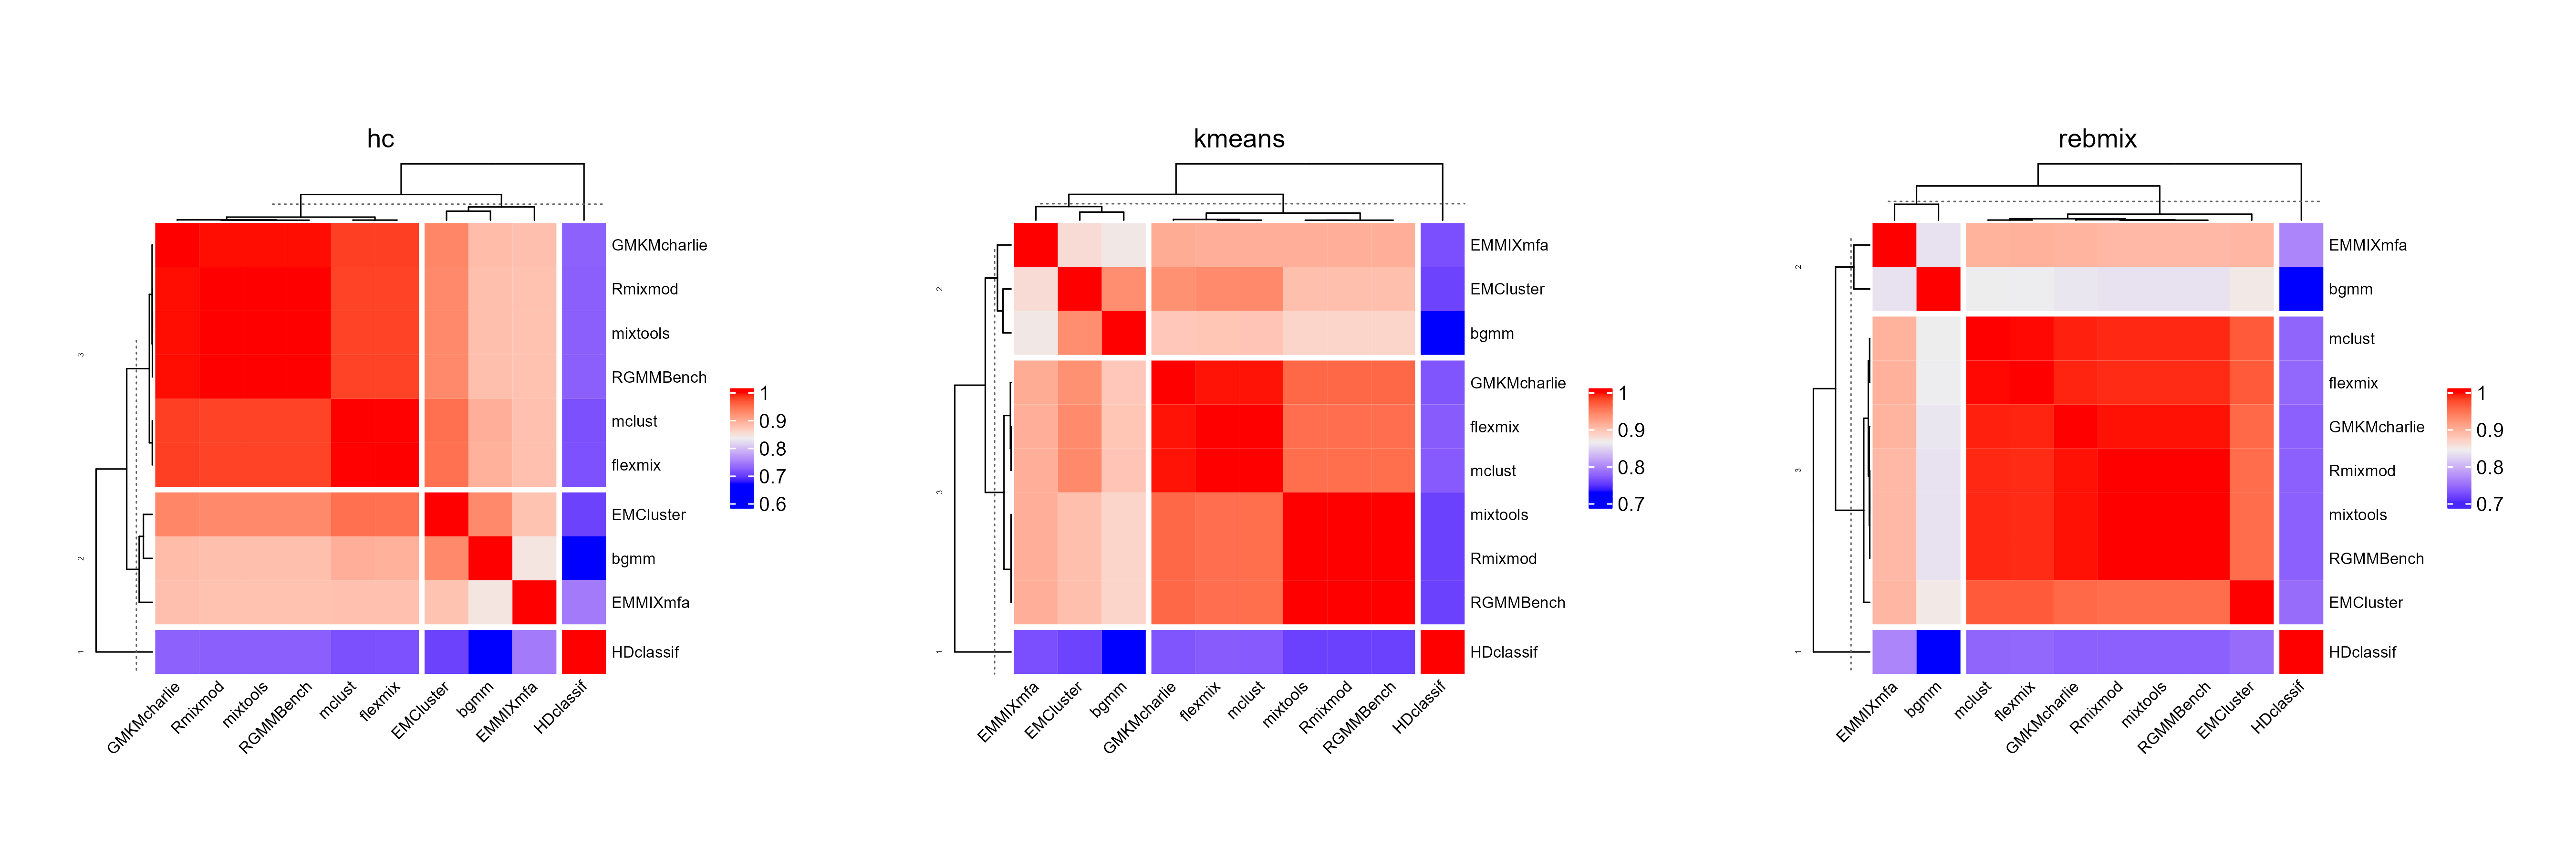
\includegraphics[width=0.8\linewidth,]{./figures/heatmap_global_HD} 

}

\caption{Correlation heatmaps of the estimated parameters in the high dimensional (HD) setting extended to the three initialisation methods benchmarked (respectively hc, \emph{k}-means and rebmix) in the most discriminating scenario HD8a).}\label{fig:heatmap-all-correlation-plots-HD}
\end{figure}


\subsection{Results description and interpretation in the high-dimensional context}
\label{results-description-and-interpretation-in-the-high-dimensional-context}

\paragraph{Unbalanced and non-overlapping components}

Scenarios HD1a-HD4b in Table \Cref{tab:parameter-configuration-HD} in the high dimensional setting, display well-separated clusters, with a representative outcome represented in Supplementary Figure \Cref{fig:HD-separated-unbalanced-ellipsoidal-plot} and Table \Cref{tab:HD-separated-unbalanced-ellipsoidal-pdf}. Consistently with results from the corresponding univariate and bivariate scenarios, most of the previously benchmarked packages return sensibly the same estimates with the hierarchical clustering and \emph{k}-means initialisation. However, \pkg{bgmm} and \pkg{EMCluster} clearly differ by lower performances with the rebmix initialisation method (however, overall, rebmix performs poorly, regardless of the package used for estimation). Notably, initialisations with the rebmix package tend to display a much larger number of poor estimations, some of which can be identified with the local maxima associated with parameter switching between the two classes. Finally, the two additional packages dedicated to high-dimensional clustering display the worst performances, with \pkg{EMMIXmfa} returning the most biased parameters and \pkg{HDclassif} the most noisy estimates. \pkg{EMMIXmfa} is the only package that returned highly biased estimates of the components' proportions in this setting.

\paragraph{Balanced and overlapping components}

In the high-dimensional scenario HD7 of Table \Cref{tab:parameter-configuration-HD}), presenting balanced but highly overlapping clusters with a full covariance structure, the best performances was obtained with \emph{k}-means initialisation, while the rebmix initialisation returns the most biased and noisy estimates. While \pkg{EMMIXmfa} performed well when it provided estimates, it returned an error in most cases (see Column \emph{Success} of Table \Cref{tab:HD-overlapping-balanced-ellipsoidal-pdf}). The least biased estimates are returned by \pkg{mixtools} and \pkg{Rmixmod} and the least noisy by \pkg{flexmix}, \pkg{mclust} and \pkg{GMKMCharlie} (smaller MSE). Interestingly, in the high-dimensional setting, the packages \pkg{EMCluster} and \pkg{bgmm} differentiate from the other packages, exhibiting worse performance. In particular, on Panel E of Figure (fig:HD-overlapping-balanced-ellipsoidal-plot), the components' proportions span the \(]0-1[^k\) simplex.
On the contrary, the \pkg{EMCluster} package, and to a lesser extent, the \pkg{bgmm} package, perform surprisingly well when datasets were simulated with an underlying spherical covariance structure, even though the estimation was not performed explicitly with this constraint (Table \Cref{tab:HD-overlapping-spherical-pdf}
). Indeed, it seems like that that the off-diagonal terms tend to converge towards 0, as showcased in Figure \Cref{fig:HD-overlapping-spherical-plot}, in Panel C, in which the fourth row from top represents the bootstrap intervals associated to the pairwise covariance between dimension 1 and 2 of each cluster.

\paragraph{Unbalanced and overlapping components}

With full covariance structures and unbalanced proportions, as depicted in the high-dimensional Scenario HD8a) and b) of Table \Cref{tab:parameter-configuration-HD}, the general observations stated in the previous subsection for the high dimensional setting hold, namely that the least biased estimates are returned by packages not specifically designed for high-dimensional data, with the \emph{k}-means initialisation (Table @ref(tab:HD-impact-num-observations-pdf-tab2 and Figure \Cref{fig:HD-impact-num-observations}). Furthermore, the pkg\{EMCluster\} and \pkg{bgmm} packages and the two packages dedicated to high-dimensional, perform similarly with \(n=200\) observations (sub-scenario a) and \(n=2000\) observations (sub-scenario b), whereas we would expect narrower and less biased confidence intervals by increasing the number of observations by a factor of 10.

Finally, with spherical covariance structures and unbalanced proportions, the best performances, both in terms of bias and variability, are obtained with \pkg{flexmix}, \pkg{mclust} and \pkg{GMKMCharlie}. Indeed, these packages are more sensitive to the choice of the initialisation method and have a greater tendency to get trapped in the neighbourhood of the initial estimates (Table \Cref{tab:HD-overlapping-spherical-pdf} and Figure \Cref{fig:HD-overlapping-spherical-plot}). Accordingly, \emph{k}-means initialisation performs best since it assumes independent and homoscedastic features for each cluster.
Furthermore, \pkg{EMMIXmfa} is the package that best estimates the off-diagonal terms in this setting, as highlighted in Table \Cref{tab:HD-overlapping-spherical-pdf-offterms}.

\paragraph{Failed estimations}

In high dimension, as tested on our third benchmark, none of the initialisations performed with the random method, carried out with \texttt{EMCluster::rand.EM()}, succeed in returning a valid parametrisation. Indeed, over the 16 scenarios tested, the covariance returned during the initialisation was systematically non-positive definite for at least one of the components, violating the properties of covariance matrices. Furthermore, as shown by the comparison of summary metrics with \(n=200\) and \(n=2000\) observations in Tables \Cref{tab:HD-impact-num-observations-pdf-tab1}
and \Cref{tab:HD-impact-num-observations-pdf-tab2}, respectively for the simplest scenario HD1 and the most complex one HD8, the rebmix initialisation on the one hand, and the packages dedicated to high dimensionality or those of the second class of packages that show a particular behaviour, present much more failures than the \emph{k}-means or hierarchical clustering initialisation, especially with the first class or the other packages of the second class.

We thus suggest not using rebmix in a high-dimensional context, displaying systematically poorer performance compared to other initialisation strategies, such as \emph{k}-means or hierarchical clustering, as illustrated by the summary metrics listed in \fullref{figures-hd-simulation}.

\section{Mixture models applied to zero-inflated distributions}
\label{sec:truncated-distribution}

\todo{detail E and M-step for truncated Gaussian mixtures + simulations with skewed Gaussian distributions}

%\section{Quasi-Gaussian distributions: skewed and excess kurtosis}